% Origen: Secciones/PI - Intro a MCA y Tipos de Usuario.md
% El archivo se llama cap6 por orden de creación, pero en template.tex va como
% primer capítulo.
\chapter{Tipos de usuario y aplicación}
\label{C:usuario}

% Figuras de ESTE capítulo + las compartidas. Siempre al principio del archivo.
\graphicspath{{figs/cap6/}{figs/comunes/}}

\begin{destacado}
En este capítulo se describe (1) la motivación de la utilización de un MCA, (2)
los pasos para poner el sistema en marcha y (3) los diferentes usos que se le
pueden dar a la aplicación desarrollada. Si contás con conocimientos previos de
espectroscopía nuclear, se recomienda ir directamente a la
Sec.~\ref{S:usr-guia}.
\end{destacado}

%==============================================================================
\section{Introducción al analizador multicanal}
\label{S:usr-mca}

Estamos constantemente expuestos a radiación, ondas electromagnéticas o
partículas subatómicas, de diversas fuentes. Las mismas pueden ser fuentes
externas a la Tierra, como los rayos cósmicos, o pueden ser internas al planeta,
por ejemplo los decaimientos de minerales en la corteza terrestre. Nuestros
sentidos no la pueden detectar de forma directa pero estas partículas tienen
interacciones físicas conocidas y medibles por dispositivos sensibles a las
mismas, estos se llaman sensores (o detectores) y nos ayudan a responder algunas
preguntas fundamentales como: \textbf{de dónde proviene la radiación y cómo está
compuesta}. La ciencia encargada de responder estas preguntas se conoce como
\textbf{espectroscopía nuclear} y resulta indispensable en campos tan diversos
como la protección radiológica de la población, la medicina nuclear, el
monitoreo ambiental, el análisis no destructivo de materiales en la industria y
la investigación científica fundamental.

En particular esta ciencia se especializa sobre los \textbf{isótopos
radiactivos} como fuentes de radiación, cada uno de estos tiene características
bien específicas, de forma que si las medimos podemos utilizarlas como
``huella'' y saber si está presente. Es en este trabajo que proponemos un
sistema electrónico capaz de medir esta ``huella'' con la mayor precisión
posible debido a que necesitamos:
\begin{enumerate}
  \item Procesar pulsos ultrarrápidos y superpuestos: podemos tener cientos de
    miles o millones de detecciones por segundo superpuestas en tiempo.
  \item Agrupar mediciones: no basta con medir un único pulso de forma aislada,
    es necesario clasificar estadísticamente miles o millones de eventos para
    obtener esta ``huella''.
  \item Determinación precisa del tiempo de medición: mientras el instrumento
    procesa un evento, queda temporalmente ``ciego'' para medir nuevos
    impulsos, tenemos que corregir este tiempo para no dar un resultado
    erróneo.
\end{enumerate}
En este paso es donde aparece el \textbf{analizador multicanal (MCA, por sus
siglas en inglés, \emph{Multichannel Analyzer})} como herramienta que realiza
estas tres tareas.

%==============================================================================
\section{Guía de usuario}
\label{S:usr-guia}

El objetivo de este trabajo fue que el sistema pudiera ser aprovechado por
usuarios con \textbf{diferentes niveles de experticia técnica}. En particular,
distinguimos tres tipos de usuarios:
\begin{enumerate}
  \item \textbf{Técnico}:
  \begin{itemize}
    \item Utiliza el sistema asumiendo que ya está calibrado y que trabaja de
      forma correcta.
    \item Sus mediciones sirven de referencia y no requieren validar la
      calibración.
    \item Se recomienda leer la Sec.~\ref{S:usr-app} y el Cap.~\ref{C:mca}.
  \end{itemize}
  \item \textbf{Calibrador}:
  \begin{itemize}
    \item Puede volver a poner un \emph{setup} experimental a punto por su cuenta: mide
      el canal analógico de la entrada y ajusta los parámetros de adquisición
      para su detector.
    \item Caracteriza el MCA con los \emph{scripts} de campaña, para saber cuánto
      confiar en las mediciones.
    \item Requiere algo de conocimiento acerca del canal analógico en la entrada
      y de los parámetros de adquisición del sistema.
    \item Se recomienda leer \textbf{todo el contenido de la tesis}.
  \end{itemize}
  \item \textbf{Desarrollador}:
  \begin{itemize}
    \item Agrega funcionalidades o cambia la estructura del HW: los parámetros de
      síntesis, la estructura del \emph{top} o de los módulos individuales, y el SW que
      los utiliza.
    \item Se recomienda leer \textbf{todo el contenido de la tesis} y referirse
      a libros de diseño digital; las fuentes del Cap.~\ref{C:intro-hw}
      contienen una buena base inicial.
  \end{itemize}
\end{enumerate}

El primero sólo quiere obtener una medición experimental, el segundo puede
cambiar los parámetros de funcionamiento del sistema de medición y el último
puede cambiar la estructura interna de los módulos y el SW que los utiliza. En la
Tabla~\ref{t:usr-guia} se presenta qué necesita cada uno: qué quiere, qué
descarga, con qué herramienta trabaja y qué conocimientos le hacen falta.

\begin{table}[H]
\centering
\caption[Guía de utilización según el tipo de usuario]{%
Guía de utilización según el tipo de usuario. La \emph{Release} contiene los
archivos para programar el HW (\emph{bitstreams}) y el SW desarrollado en este
proyecto.\label{t:usr-guia}}
\begin{tabularx}{\textwidth}{|>{\raggedright\arraybackslash}p{0.17\textwidth}%
  |>{\raggedright\arraybackslash}X|>{\raggedright\arraybackslash}X%
  |>{\raggedright\arraybackslash}p{0.2\textwidth}|}
\hline \encabezado \textbf{Tipo de usuario} & \textbf{Objetivo principal} &
  \textbf{Herramienta y enfoque recomendado} & \textbf{Requiere} \\ \hline
\textbf{Técnico} & Realizar mediciones de espectrometría estándar con el
  sistema ya calibrado. & Uso directo de la aplicación gráfica cliente
  (\codigo{mcamon}) en modo operacional, sin requerir conocimientos de
  programación. & \textbf{\emph{Release}} (5,0~MB) \\ \hline
\textbf{Calibrador} & Poner a punto un \emph{setup} experimental, caracterizar
  el canal analógico y ajustar parámetros de adquisición. & Uso de la interfaz
  completa con la pestaña de \emph{Calibration} y ejecución de \emph{scripts} de
  automatización en Python. & \textbf{\emph{Release}} (5,0~MB) \\ \hline
\textbf{Desarrollador} & Modificar o extender la lógica del hardware
  reconfigurable (RTL) o la API del sistema. & Acceso al repositorio completo,
  entorno de síntesis en Vivado y desarrollo de software embebido en C/Python.
  & \textbf{Repositorio completo} (537~MB) y \textbf{Vivado 2020.1} (25~GB)
  \\ \hline
\end{tabularx}
\end{table}

El Calibrador que quiera actualizar el software en la placa con \cmd|git pull|
puede bajar, en lugar de la \emph{Release}, un clon parcial del repositorio (31~MB) con
sólo el software, la documentación y los \emph{bitstreams}; en ese caso necesita un
conocimiento básico de Git.

\subsection{Pasos requeridos para la utilización}
\label{S:usr-pasos}

El Técnico y el Calibrador trabajan con la \emph{Release} del
repositorio~\cite{RepoReleases}, un paquete con los \emph{bitstreams} y el software que
salieron del mismo \emph{commit}. Que viajen juntos importa: un \emph{bitstream} viejo ignora
en silencio las escrituras a los registros que no conoce, así que un software
nuevo puede no fallar y medir números plausibles y equivocados.

En la placa:
\begin{enumerate}
  \item Conectar la placa de desarrollo a la red y la señal del detector a la
    entrada IN1. Ir a la guía de inicio de Red
    Pitaya~\cite{RedPitayaQuickStart} si se encuentra algún problema.
  \item Acceder a la placa mediante un cliente SSH.
  \item Descargar la \emph{Release} dentro de la placa, descomprimirla e instalarla con
    el comando de abajo, que además programa la PL y verifica que los
    registros del MCA respondan:
\begin{comando}
sudo ./instalar.sh --cargar
\end{comando}

  \item Comprobar que la PL quedó programada con el \emph{bitstream} de la \emph{Release}:
\begin{comando}
python3 /opt/mca/software/campanas/preparar_placa.py
\end{comando}

  \item Iniciar el servidor de control remoto:
\begin{comando}
sudo python3 /opt/mca/software/app/mca_server.py --port 1001
\end{comando}

\end{enumerate}

En la PC:
\begin{enumerate}[resume]
  \item Descargar la \emph{Release}, descomprimirla e instalar las dependencias del
    cliente:
\begin{comando}
pip install PyQt5 matplotlib numpy
\end{comando}

  \item Iniciar el cliente desde \ruta{software/}:
\begin{comando}
python3 app/mcamon.py --host <ip-de-la-pitaya> --port 1001 --conectar
\end{comando}

\end{enumerate}

% sloppypar: los \verb no se cortan y el renglón se pasaba 5 pt.
\begin{sloppypar}
Antes de tener la placa, la APP puede probarse contra un MCA simulado con
\cmd|make app-demo|, que levanta un servidor falso y el cliente en la misma PC.
El Desarrollador, con el repositorio completo, hace los pasos 5 a 7 desde la PC
con \cmd|make app| dentro de \ruta{prj/MCA}: sincroniza el software con la
placa, levanta el servidor y abre el cliente.
\end{sloppypar}

%==============================================================================
\section{Aplicación cliente en Python}
\label{S:usr-app}

Nos basamos en la aplicación mcpha desarrollada por Pavel
Demin~\cite{DeminMCPHA}, que funciona en modalidad servidor-cliente con
comunicación por \emph{sockets} de red; en la Fig.~\ref{f:usr-mcpha} se observa una
captura. La misma cuenta con:
\begin{itemize}
  \item Un servidor programado en C, que:
  \begin{itemize}
    \item Corre en el PS de la Red Pitaya y lee de la PL los histogramas de su MCA.
    \item Implementa un protocolo de comunicación propio.
  \end{itemize}
  \item Un cliente programado en Python, que:
  \begin{itemize}
    \item Parsea los paquetes recibidos según ese protocolo.
    \item Corre una GUI desarrollada en PyQt5.
    \item Cuenta con las opciones de:
    \begin{itemize}
      \item Manejo de conexión.
      \item Representación gráfica interactiva del histograma mediante
        matplotlib.
      \item Reporte de cantidad de cuentas.
      \item Control de adquisición.
    \end{itemize}
  \end{itemize}
\end{itemize}

\begin{figure}[H]
\centering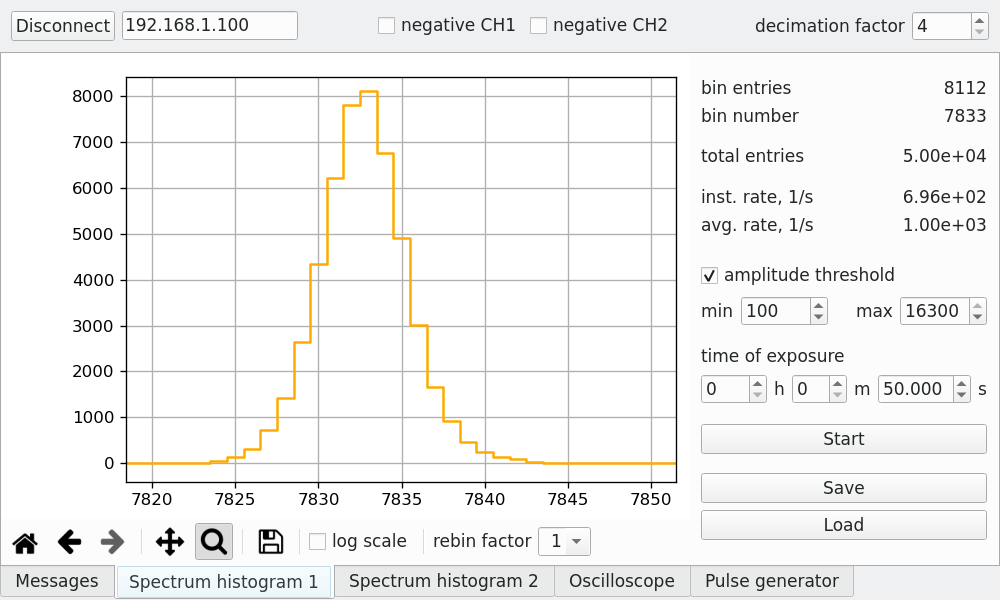
\includegraphics{cap6_mcpha_client}
\caption[GUI de mcpha, de Pavel Demin]{%
Captura de pantalla de la GUI de mcpha, implementada por Pavel Demin para su
versión del MCA~\cite{DeminMCPHA}.\label{f:usr-mcpha}}
\end{figure}

La aplicación realizada en este trabajo, \codigo{mcamon} (por \emph{MCA
monitor}), es una adaptación de esta GUI al HW y SW de este proyecto. Se controla
desde un cliente externo conectado por red, escrito con PyQt5 y matplotlib, que
se conecta con el servidor \codigo{mca\_server.py}. A diferencia de mcpha, el
servidor está escrito en Python: corre en la placa, llama a la API de
adquisición y responde con el protocolo de la Sec.~\ref{S:sw-protocolo-red}.

Casi todas las diferencias con mcpha las imponen los módulos del hardware, que
no es el mismo; se presentan en la Tabla~\ref{t:usr-diferencias-mcpha}.

% [H]: es lo último del capítulo; como float quedaba solo detrás de las referencias.
\begin{table}[H]
\centering
\caption[Diferencias entre mcpha y la aplicación de este trabajo]{%
Diferencias entre mcpha y la aplicación de este
trabajo.\label{t:usr-diferencias-mcpha}}
\begin{tabularx}{\textwidth}{|>{\raggedright\arraybackslash}p{0.36\textwidth}%
  |>{\raggedright\arraybackslash}X|}
\hline \encabezado \textbf{mcpha} & \textbf{Este trabajo} \\ \hline
Dos MCA independientes, con una pestaña de espectro cada uno & Un solo MCA, con
  un selector de canal IN1/IN2 \\ \hline
4096 canales fijos & La cantidad de canales se lee del hardware (registro
  \codigo{WIDTHS}); el cliente no la supone \\ \hline
Temporizador de exposición en hardware & Lo implementa un hilo del servidor,
  contra el tiempo vivo \\ \hline
Negador por canal & No hay negador; en su lugar se elige si la amplitud es el
  pico o la integral de carga \\ \hline
--- & Contadores propios:\newline
  \textbullet~Rechazados por amplitud y por forma.\newline
  \textbullet~Apilados y disparos perdidos.\newline
  \textbullet~Tiempos real, vivo y muerto. \\ \hline
--- & Mapa 2D de forma de pulso y su figura de mérito \\ \hline
\end{tabularx}
\end{table}

La interfaz está en inglés y trae las pestañas de la
Tabla~\ref{t:usr-pestanas}; algunas aparecen sólo si el \emph{bitstream} cargado trae el
módulo correspondiente.

% [H]: es lo último del capítulo; como float quedaba solo detrás de las referencias.
\begin{table}[H]
\centering
\caption[Pestañas de la aplicación y su contenido]{%
Pestañas de la aplicación y su contenido.\label{t:usr-pestanas}}
\begin{tabularx}{\textwidth}{|>{\raggedright\arraybackslash}p{0.2\textwidth}%
  |>{\raggedright\arraybackslash}X|}
\hline \encabezado \textbf{Pestaña} & \textbf{Qué contiene} \\ \hline
\textbf{\emph{Messages}} & cada operación y cada error, con su hora \\ \hline
\textbf{\emph{Spectrum}} & el histograma 1D; la tasa de entrada instantánea y media;
  los contadores (aceptados, rechazados, apilados, perdidos); el tiempo real,
  vivo y muerto; los botones \emph{Start}, \emph{Stop}, \emph{Clear} y de guardado; la lista de picos
  con su FWHM y resolución \\ \hline
\textbf{MCA \emph{settings}} & la franja del MCA, con la tasa y las pérdidas de cada
  etapa; abajo, los registros agrupados por función: preprocesamiento,
  segmentación y ranuras, publicación \\ \hline
\textbf{2D \emph{map} (PSD)} & el mapa de amplitud $\times$ factor de forma
  ($Q_\text{tail}/Q_\text{total}$) y la figura de mérito \\ \hline
\textbf{\emph{Integration}} & de qué punto de la cadena de procesamiento toma sus
  muestras cada consumidor (OSC, multitrigger, MCA, \codigo{event\_ring}) y el
  control global de todo el sistema (\emph{run}, \emph{clear}, \emph{reset}) \\ \hline
\textbf{\emph{Pulses}} & las capturas del osciloscopio, como pulso o como mapa de
  calor, y la tasa en el tiempo \\ \hline
\textbf{OSC \emph{settings}} & la franja del osciloscopio (y la del \emph{ring}, si el
  \emph{bitstream} lo trae), los registros por etapa y la adquisición del \emph{ring} a una
  carpeta de la placa \\ \hline
\textbf{Multitrigger} & la franja del disparo: las fuentes (nivel, pendiente,
  polo-cero), las máscaras OR por canal y el \emph{shield} \\ \hline
\textbf{\emph{Generator}} & el generador de pulsos por etapas (disparos, amplitud,
  forma, salida) y el lazo digital hacia el MCA \\ \hline
\textbf{\emph{Calibration}} & la medición del canal analógico con una referencia
  conocida (\emph{offset}, ruido, ganancia, caída lenta, ancho de banda, diafonía) y la
  base dinámica del MCA \\ \hline
\end{tabularx}
\end{table}

En el Apéndice~\ref{C:ap-app} aparecen capturas de cada una de las pestañas.

% Bibliografía de este capítulo. Va al final del archivo, siempre.
\bibliografiacapitulo

%%% Local Variables:
%%% mode: latex
%%% TeX-master: "template"
%%% End:
